\documentclass{beamer}
\usepackage[utf8]{inputenc}

\usetheme{Boadilla}
\usecolortheme{lily}
\usepackage{amsmath,amssymb,amsfonts,amsthm}
\usepackage{mathtools}
\usepackage{txfonts}
\usepackage{tkz-euclide}
\usepackage{listings}
\usepackage{adjustbox}
\usepackage{array}
\usepackage{tabularx}
\usepackage{lmodern}
\usepackage{circuitikz}
\usepackage{tikz}
\usepackage{graphicx}

\setbeamertemplate{footline}
{
  \leavevmode%
  \hbox{%
  \begin{beamercolorbox}[wd=\paperwidth,ht=2.25ex,dp=1ex,right]{author in head/foot}%
    \insertframenumber{} / \inserttotalframenumber\hspace*{2ex} 
  \end{beamercolorbox}}%
  \vskip0pt%
}

\usepackage{tcolorbox}
\tcbuselibrary{minted,breakable,xparse,skins}




\providecommand{\nCr}[2]{\,^{#1}C_{#2}} % nCr
\providecommand{\nPr}[2]{\,^{#1}P_{#2}} % nPr
\providecommand{\mbf}{\mathbf}
\providecommand{\pr}[1]{\ensuremath{\Pr\left(#1\right)}}
\providecommand{\qfunc}[1]{\ensuremath{Q\left(#1\right)}}
\providecommand{\sbrak}[1]{\ensuremath{{}\left[#1\right]}}
\providecommand{\lsbrak}[1]{\ensuremath{{}\left[#1\right.}}
\providecommand{\rsbrak}[1]{\ensuremath{{}\left.#1\right]}}
\providecommand{\brak}[1]{\ensuremath{\left(#1\right)}}
\providecommand{\lbrak}[1]{\ensuremath{\left(#1\right.}}
\providecommand{\rbrak}[1]{\ensuremath{\left.#1\right)}}
\providecommand{\cbrak}[1]{\ensuremath{\left\{#1\right\}}}
\providecommand{\lcbrak}[1]{\ensuremath{\left\{#1\right.}}
\providecommand{\rcbrak}[1]{\ensuremath{\left.#1\right\}}}
\theoremstyle{remark}
\newtheorem{rem}{Remark}
\newcommand{\sgn}{\mathop{\mathrm{sgn}}}
\providecommand{\abs}[1]{\left\vert#1\right\vert}
\providecommand{\res}[1]{\Res\displaylimits_{#1}} 
\providecommand{\norm}[1]{\lVert#1\rVert}
\providecommand{\mtx}[1]{\mathbf{#1}}
\providecommand{\mean}[1]{E\left[ #1 \right]}
\providecommand{\fourier}{\overset{\mathcal{F}}{ \rightleftharpoons}}
%\providecommand{\hilbert}{\overset{\mathcal{H}}{ \rightleftharpoons}}
\providecommand{\system}{\overset{\mathcal{H}}{ \longleftrightarrow}}
	%\newcommand{\solution}[2]{\textbf{Solution:}{#1}}
%\newcommand{\solution}{\noindent \textbf{Solution: }}
\providecommand{\dec}[2]{\ensuremath{\overset{#1}{\underset{#2}{\gtrless}}}}
\newcommand{\myvec}[1]{\ensuremath{\begin{pmatrix}#1\end{pmatrix}}}
\let\vec\mathbf

\lstset{
%language=C,
frame=single, 
breaklines=true,
columns=fullflexible
}

\numberwithin{equation}{section}

\lstset{
  language=Python,
  basicstyle=\ttfamily\small,
  keywordstyle=\color{blue},
  stringstyle=\color{orange},
  numbers=left,
  numberstyle=\tiny\color{gray},
  breaklines=true,
  showstringspaces=false
}

\title{Problem 4.11.1}
\author{ee25btech11023-Venkata Sai}

\date{\today} 
\begin{document}

\begin{frame}
\titlepage
\end{frame}

\section*{Outline}
\begin{frame}
\tableofcontents
\end{frame}

\section{Problem}

\begin{frame}
\frametitle{Problem}
Find the coordinates of the point where the line  $\frac{x-1}{3} = \frac{y+4}{7} = \frac{z+4}{2}$ cuts the XY-plane 
\end{frame}
%\subsection{Literature}
\section{Solution}

\subsection{Declaration of variables}
\begin{frame}
\setcounter{section}{1}
\frametitle{Declaration of variables}
The line equation is  
\begin{align}
\vec{r} = \vec{a} + t \vec{b}
\end{align}
where $\vec{a}$ is the point on line and $\vec{b}$ is the direction vector
\begin{align}
\vec{a} = \myvec{1 \\ -4 \\ -4}\ \text{and}\
\vec{b} = \myvec{3 \\ 7 \\ 2}
\end{align}
The normal vector to XY plane is
\begin{align}
\vec{n} = \myvec{0 \\ 0 \\ 1}
\end{align}
The plane equation of the XY-plane is  
\begin{align}
\vec{n}^T \vec{x} = 0 \implies \myvec{0 & 0 & 1}\vec{x}=0
\end{align}
\end{frame}
\subsection{Solving}
\begin{frame}
\frametitle{Solving}
 Substituting the line into the plane equation gives  
\begin{align}
\vec{n}^T\brak{ \vec{a} + t\vec{b}} = 0  \\
\vec{n}^T \vec{a} + t\brak{\vec{n}^T \vec{b}} = 0 \\
t\brak{\vec{n}^T \vec{b}}=-\vec{n}^T \vec{a} 
\end{align}
\begin{align}
t =-\frac{\vec{n}^T \vec{a}}{\vec{n}^T \vec{b}}
\end{align}
\begin{align}
t =-\frac{\myvec{0 & 0 & 1}\myvec{1 \\ -4 \\ -4}}{\myvec{0 & 0 & 1}\myvec{3 \\ 7 \\ 2}}  = -\frac{-4}{2} 
\end{align}
\begin{align}
\implies t=2
\end{align}
\end{frame}
\subsection{Conclusion}
\begin{frame}
\frametitle{Conclusion}
The intersection point is  
\begin{align}
\vec{r} = \vec{a} + t\vec{b} 
= \myvec{1 \\ -4 \\ -4} + 2\myvec{3 \\ 7 \\ 2}
\end{align} 
\begin{align}
\vec{r} = \myvec{7 \\ 10 \\ 0}
\end{align}
\end{frame}

\subsection{Plot}
\begin{frame}[fragile]
\frametitle{Plot}

\begin{figure}[h!]
   \centering
   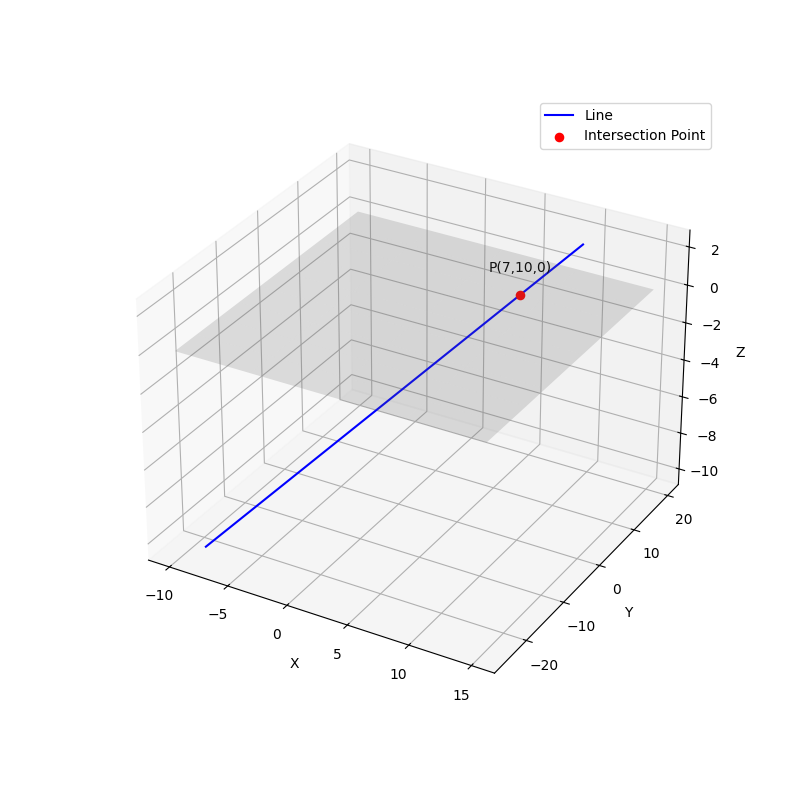
\includegraphics[width=0.7\columnwidth]{figs/fig1.png}
	\caption{}
   \label{}
\end{figure}
\end{frame}

\section{C Code}
\begin{frame}[fragile]
\frametitle{C Code}
\begin{lstlisting}[language=C]
void get_intersection_data(double* out_data) {
    double point_a[3] = {1.0, -4.0, -4.0};
    double dir_d[3] = {3.0, 7.0, 2.0};
    double lambda = 2.0;

    double Px = point_a[0] + lambda * dir_d[0]; 
    double Py = point_a[1] + lambda * dir_d[1]; 
    double Pz = point_a[2] + lambda * dir_d[2]; 
 
    out_data[0] = Px; 
    out_data[1] = Py; 
    out_data[2] = Pz;
    out_data[3] = point_a[0];
    out_data[4] = point_a[1]; 
    out_data[5] = point_a[2];
    out_data[6] = dir_d[0]; 
    out_data[7] = dir_d[1]; 
    out_data[8] = dir_d[2];
}
    \end{lstlisting}
\end{frame}
\section{Python Code}
\begin{frame}[fragile]
\frametitle{Python Code for Calling}
\begin{lstlisting}[language=Python]
import ctypes
import numpy as np

def get_line_data_from_c():

    lib = ctypes.CDLL('./coord.so')
    double_array_9 = ctypes.c_double * 9
    lib.get_intersection_data.argtypes = [ctypes.POINTER(ctypes.c_double)]

    out_data_c = double_array_9()
    lib.get_intersection_data(out_data_c)
    all_data = np.array(out_data_c)
    # Split the data into the three vectors
    intersection_P = all_data[0:3]
    point_a = all_data[3:6]
    dir_d = all_data[6:9]
    
    return intersection_P, point_a, dir_d
\end{lstlisting}
\end{frame}
\begin{frame}[fragile]
\frametitle{Python Code for Plotting}
\begin{lstlisting}[language=Python]
#Code by GVV Sharma
#September 12, 2023
#Revised July 21, 2024
#released under GNU GPL
import sys                                          #for path to external scripts
sys.path.insert(0, '/workspaces/urban-potato/matgeo/codes/CoordGeo/') 
import numpy as np
import matplotlib.pyplot as plt
from mpl_toolkits.mplot3d import Axes3D

#local imports
from line.funcs import *
from triangle.funcs import *

from call import get_line_data_from_c
\end{lstlisting}
\end{frame}

\begin{frame}[fragile]
\frametitle{Python Code for Plotting}
\begin{lstlisting}[language=Python]
P, point_a, dir_d = get_line_data_from_c()
 line_points=point_a+np.array([-3,3]).reshape(-1,1)*dir_d
fig=plt.figure(figsize=(8,8))
ax=fig.add_subplot(111,projection='3d')
X_plane=np.linspace(-10,15,5)
Y_plane=np.linspace(-25,20,10)
X_plane,Y_plane = np.meshgrid(X_plane,Y_plane)
Z_plane=np.zeros_like(X_plane)
ax.plot_surface(X_plane,Y_plane,Z_plane,alpha=0.2,color='gray')
ax.plot(line_points[:,0],line_points[:,1],line_points[:,2],color='b',label='Line')
\end{lstlisting}
\end{frame}

\begin{frame}[fragile]
\frametitle{Python Code for Plotting}
\begin{lstlisting}[language=Python] 
ax.scatter(P[0], P[1], P[2], color='r', s=35, label='Intersection Point')
ax.text(P[0], P[1], P[2] + 1.2, f'P({P[0]:.0f}, {P[1]:.0f}, {P[2]:.0f})', ha='center')

ax.set_title('Intersection of a Line with the XY Plane')
ax.set_xlabel('X-axis')
ax.set_ylabel('Y-axis')
ax.set_zlabel('Z-axis')
ax.legend()
plt.show()
plt.savefig('../figs/fig1.png')
\end{lstlisting}
\end{frame}

\end{document}
